
Resistive forces on one-dimensional oscillators is common. For instance, friction along a surface for a mass of a spring. For sanitys sake, we study the force being proportional to $v$ only. It is assumed the resistive force looks like $\vec{f} = -b\vec{v}$. Isolating the terms in the equation of motion (one-dimensional Newton's 2nd law, resistive force, and Hooke's law) yields,

\begin{equation}
    m\ddot{x} + b\dot{x} + kx = 0
    \label{eqn:damped_oscillator}
\end{equation}

Equation \ref{eqn:damped_oscillator} also shows up in the study of LRC circuits (more on those later).

The introduction of some constants is necessary before equation \ref{eqn:damped_oscillator} is solved. Replacing $2\beta = \frac{b}{m}$ as a convenient {\bfseries damping constant} (high $\beta$, high damping) and $\omega_o^2$ with $\frac{k}{m}$, where $\omega_o$ is the {\bfseries natural frequency} or the frequency at which it would oscillate if there were no resistive force present. The equation of motion then becomes,

\begin{equation}
    \ddot{x} + 2\beta \dot{x} + \omega_o^2 x = 0.
    \label{eqn:damped_oscillator2}
\end{equation}

This equation is a second-order, linear, homogeneous equation (like regular oscillator) and take inspired guesses for a solution. Trying the solution $x(t) = e^{rt}$ yields $\dot{x}(t) = re^{rt}$ and $\ddot{x}(t) = r^2e^{rt}$. These solutions only work if the auxiliary equation is

\begin{equation*}
    r^2 + 2\beta r + \omega_o^2 = 0.
\end{equation*}

The solution to this equation is, by use of the quadratic equation, $r = -\beta \pm \sqrt{\beta^2 - \omega_o^2}$. The two independent solutions ($r_1 \rightarrow +$ and $r_2 \rightarrow -$) for a general solution through addition:

\begin{gather*}
    x(t) = C_1 e^{r_1 t} + C_2 e^{r_2 t} \\
    x(t) = e^{-\beta t} (C_1 e^{\sqrt{\beta^2 - \omega_o^2}t} + C_2 e^{-\sqrt{\beta^2 - \omega_o^2}t})
\end{gather*}

Examining this equation with different damping constants $\beta$ illuminate the scenarios of damped oscillators.


{\vspace{0.35cm} \bfseries \noindent Undamped oscillators}

Replacing $\beta$ with zero yields (thru $\sqrt{-}$) the familiar solution to an undamped harmonic oscillator,

\begin{equation*}
    x(t) = C_1 e^{i \omega_o^ t} + C_2 e^{-i \omega_o^ t}
\end{equation*}


{\vspace{0.35cm} \bfseries \noindent Weak damping}

The condition that $\beta < \omega_o$ is sometimes called {\bfseries underdamping}. The square root again becomes imaginary $\sqrt{\beta^2 - \omega_o^2} = i\sqrt{\omega_o^2 - \beta^2} = i \omega_1$ where $\omega_1$ is a frequency that is less than the natural frequency. The solution then becomes,

\begin{equation*}
    x(t) = e^{-\beta t} (C_1 e^{\omega_1 t} + C_2 e^{-\omega_1 t})
\end{equation*}

The second term here can be solved into the form,

\begin{equation*}
    x(t) = A e^{-\beta t} cos(\omega_1 t - \delta).
\end{equation*}

This is obviously a simple harmonic motion of frequency $\omega_!$ with a decaying factor $A e^{-\beta t}$. The result is shown in figure \ref{fig:weak_damped_osc}. A decay parameter (a measure of the rate at which the motion dies out) can be characterized as $\beta$.

\begin{figure}[h]
    \centering
    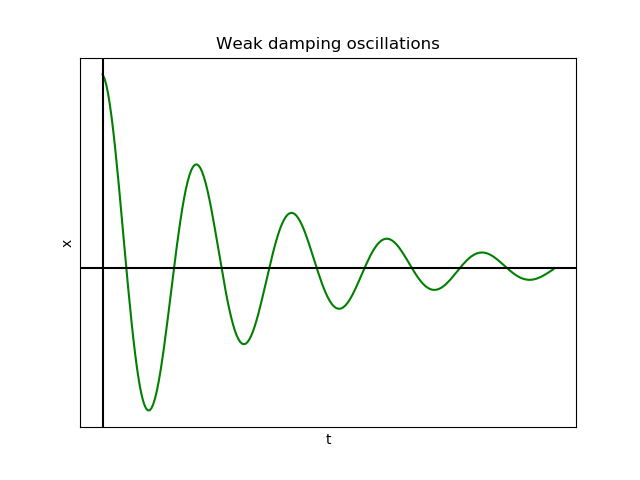
\includegraphics[width=8cm]{Classical_Mechanics/2.12-damp-osc/weak_damped_osc.png}
    \caption{As $t \rightarrow \infty$, $x \rightarrow 0$ (equilibrium) while oscillating over the equilibrium repeatedly.}
    \label{fig:weak_damped_osc}
\end{figure}


{\vspace{0.35cm} \bfseries \noindent Strong damping}

Suppose that $\beta$ is large, specifically that $\beta > \omega_o$. This condition is sometimes called {\bfseries overdamping}. The square roots and exponents are real and our solution is,

\begin{equation*}
    x(t) = C_1 e^{-(\beta - \sqrt{\beta^2 -\omega_o^2}) t} + C_2 e^{-(\beta + \sqrt{\beta^2 -\omega_o^2}) t}
\end{equation*}

This motion is shown in figure \ref{fig:strong_damped_osc}. The decay parameter is characterized by the coefficient of the first exponent, $\beta - \sqrt{\beta^2 - \omega_o^2}$.

\begin{figure}[h]
    \centering
    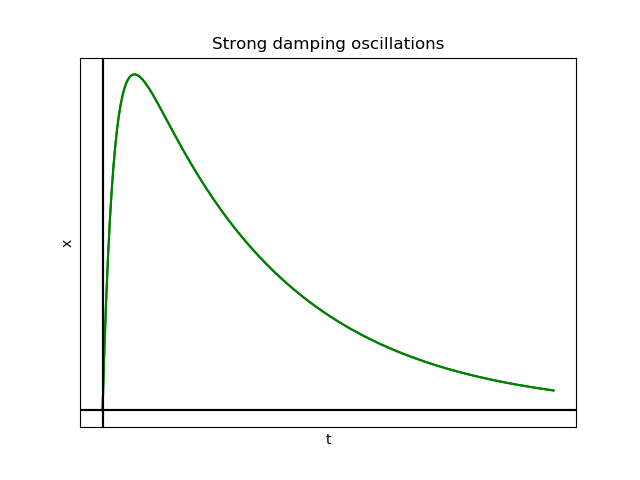
\includegraphics[width=8cm]{Classical_Mechanics/2.12-damp-osc/strong_damped_osc.png}
    \caption{As $t \rightarrow \infty$, $x \rightarrow 0$ (equilibrium) from one side only.}
    \label{fig:strong_damped_osc}
\end{figure}


{\vspace{0.35cm} \bfseries \noindent Critical damping}

Critical damping occurs when $\beta = \omega_o$. The general solution for this case is

\begin{equation*}
    x(t) = C_1 e^{-\beta t} + C_2 t e^{-\beta t}.
\end{equation*}

The decay parameter here is $\beta = \omega_o$. The decay parameter information is condensed to the table below.

\vspace{0.35cm}

\begin{table}[h]
    \centering
    \begin{tabular}{c c c}
        damping & $\beta$ & decay parameter\\
        \hline
        none & $\beta = 0$ & 0\\
        under & $\beta < \omega_o$ & $\beta$ \\
        critical & $\beta = \omega_o$ & $\beta$ \\
        over & $\beta > \omega_o$ & $\beta - \sqrt{\beta^2 - \omega_o^2}$.
    \end{tabular}
\end{table}


{\exbegin}

In order to keep a decaying oscillation oscillating, it needs to be driven by an external force, much like any natural oscillator. Accounting for this "driving" force is as simple as changing equation \ref{eqn:damped_oscillator} to

\begin{equation*}
    m\ddot{x} + b\dot{x} + kx = F(t),
\end{equation*}

\noindent where $F(t)$ is the driving force varying with time. Similar to its non-driven counterpart, this equation is simplified in the same manner as equation \ref{eqn:damped_oscillator2} was: dividing everything by $m$ and replacing $b/m$ with $2\beta$ and $k/m$ with $\omega_o^2$. Thus,

\begin{equation*}
    \ddot{x} + 2\beta \dot{x} + \omega_o^2 x = \frac{F(t)}{m},
\end{equation*}

This section may require a dust-off of linear differential operators. See the appropriate subsection in Miscellaneous Topics for this review.

We find the homogenous solution above in the undriven damped oscillator: $x_h = C_1e^{r_1t} + C_2e^{r_2t}$. The general solution is such that $x_h + x_p$, where $x_p$ is the particular solution. Find a particular solution, get the general solution. Easy enough.

To help understand this, look at an example of a sinusoidal driving force,

\begin{equation*}
    \frac{F(t)}{m} = f(t) = f_0 cos(\omega t),
\end{equation*}

\noindent where $f_0$ is the driving force amplitude (divided by mass still) and $\omega$ is the driving frequency (not the natural frequency $\omega_o$!). The equation of motion then becomes,

\begin{equation*}
    \ddot{x} + 2\beta \dot{x} + \omega_o^2 x = f_0 cost(\omega t).
\end{equation*}

Through magic (complex numbers [$z$]), the particular solution is, $z(t) = Ce^{i \omega t}$ when $C = \frac{f_0}{\omega_o^2 - \omega^2 + 2i\beta \omega}$. Turning our solution into a complex number and taking the real part only is at the heart of Fourier transforms. This real part yields,

\begin{equation*}
    x_p(t) = A cos(\omega t - \delta)
\end{equation*}

\noindent where,

\begin{gather*}
    A^2 = \frac{f_0^2}{(\omega_o^2 - \omega^2)^2 + 4\beta^2\omega^2} \\
    \delta = arctan(\frac{2\beta\omega}{\omega_o^2 - \omega^2}).
\end{gather*}

Recalling that the general solution is the sum of a particular and the homogeneous solution, the general solution becomes,

\begin{equation*}
    x(t) = x_p(t) + x_h(t) = A cos(\omega t - \delta) + C_1e^{r_1t} + C_2e^{r_2t}.
\end{equation*}

\noindent The two extra terms die out exponentially as time increases, so they are called {\itshape transients}. They depend on initial conditions but eventually become irrelevant. See figure \ref{fig:driving_osc} for more details.

\begin{figure}[h]
    \centering
    \begin{subfigure}[t]{0.4\textwidth}
        \centering
        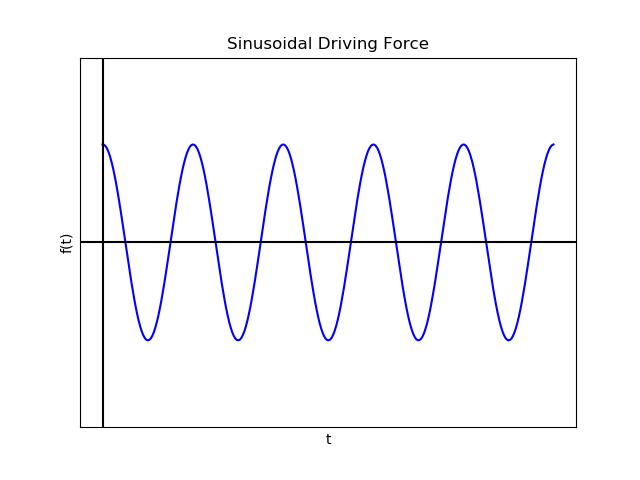
\includegraphics[width=6.5cm]{Classical_Mechanics/2.12-damp-osc/driven_osc_force.png}
        \caption{The sinusoidal driving force $f(t) = Acos(\omega t - \delta)$ is shown here.}
    \end{subfigure}
    ~ 
    \begin{subfigure}[t]{0.4\textwidth}
        \centering
        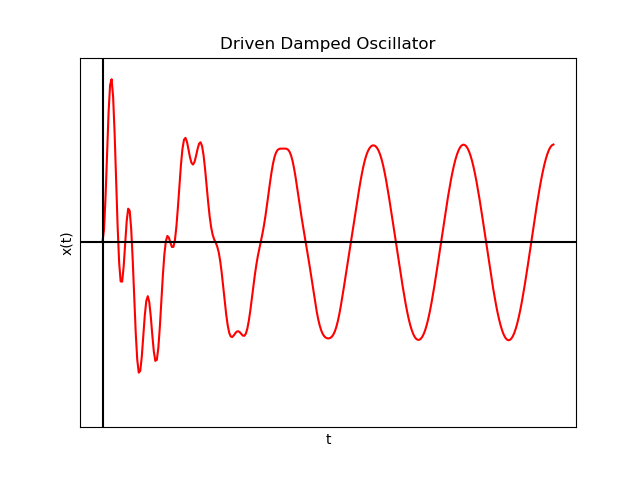
\includegraphics[width=6.5cm]{Classical_Mechanics/2.12-damp-osc/driven_damped_osc1.png}
        \caption{The resultant driven oscillation. Note the transient forces becoming non-existent after a couple oscillations.}
    \end{subfigure}
    \caption{An example of a driven damped oscillation.}
    \label{fig:driving_osc}
\end{figure}